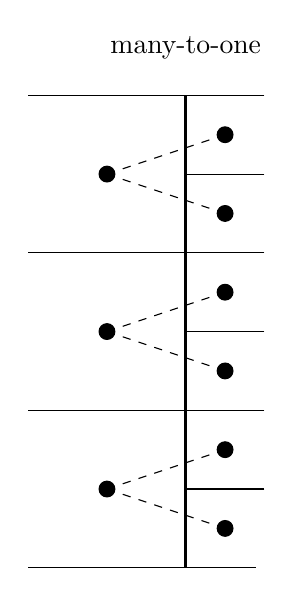
\begin{tikzpicture}[scale=2.0]

\coordinate (P1) at (0,0);
\coordinate (P2) at (0,0.5);
\coordinate (P3) at (0,1);
\coordinate (P4) at (0,1.5);
\coordinate (P5) at (0,2);
\coordinate (P6) at (0,2.5);
\coordinate (P7) at (0,3);

\draw[very thick] (P1) -- (P7);

\coordinate (L1) at (-1,0);
\coordinate (L2) at (-1,1);
\coordinate (L3) at (-1,2);
\coordinate (L4) at (-1,3);

\coordinate (LL1) at (barycentric cs:P1=1,P3=1,L1=1,L2=1);
\coordinate (LL2) at (barycentric cs:P3=1,P5=1,L2=1,L3=1);
\coordinate (LL3) at (barycentric cs:P5=1,P7=1,L3=1,L4=1);

\coordinate (R1) at (0.5,0);
\coordinate (R2) at (0.5,0.5);
\coordinate (R3) at (0.5,1);
\coordinate (R4) at (0.5,1.5);
\coordinate (R5) at (0.5,2);
\coordinate (R6) at (0.5,2.5);
\coordinate (R7) at (0.5,3);

\coordinate (RR1) at (barycentric cs:P1=1,P2=1,R1=1,R2=1);
\coordinate (RR2) at (barycentric cs:P2=1,P3=1,R2=1,R3=1);
\coordinate (RR3) at (barycentric cs:P3=1,P4=1,R3=1,R4=1);
\coordinate (RR4) at (barycentric cs:P4=1,P5=1,R4=1,R5=1);
\coordinate (RR5) at (barycentric cs:P5=1,P6=1,R5=1,R6=1);
\coordinate (RR6) at (barycentric cs:P6=1,P7=1,R6=1,R7=1);

\foreach \i in {1,2,3}
{
  \draw[fill=black] (LL\i) circle (0.05);
}

\foreach \i in {1,2,3,4,5,6}
{
  \draw[fill=black] (RR\i) circle (0.05);
}

\draw (L1) -- (P1);
\draw (L2) -- (P3);
\draw (L3) -- (P5);
\draw (L4) -- (P7);

\draw (R1) -- (P1);
\draw (R2) -- (P2);
\draw (R3) -- (P3);
\draw (R4) -- (P4);
\draw (R5) -- (P5);
\draw (R6) -- (P6);
\draw (R7) -- (P7);

\draw[dashed] (LL1) -- (RR1);
\draw[dashed] (LL1) -- (RR2);
\draw[dashed] (LL2) -- (RR3);
\draw[dashed] (LL2) -- (RR4);
\draw[dashed] (LL3) -- (RR5);
\draw[dashed] (LL3) -- (RR6);

\node[align=left] at (0,+3.3) {many-to-one};

\draw[fill=white,white] (0.5,0) circle (0.05);

\end{tikzpicture}
